\documentclass[]{scrartcl}
\title{Vorlesung Analysis II}
\usepackage{amsmath,amssymb,amsfonts}
\usepackage{mathtools}
\usepackage{graphicx}
\usepackage{tikz}
\usepackage{xcolor}
\usepackage{soul}
\usepackage{hyperref}
\usepackage{tipa}
\hypersetup{
	colorlinks=true,
	linkcolor=blue,
	filecolor=magenta,      
	urlcolor=cyan,
	pdftitle={Overleaf Example},
	pdfpagemode=FullScreen,
}
\newcommand{\redcircle}[1]{%
	\tikz[baseline=(char.base)]{
		\node[shape=circle, draw=red, text=red, thick, inner sep=1pt] (char) 
		{\textbf{#1}};
	}%
}
\setul{1pt}{3pt} % Linienhöhe und Abstand zum Text (optional anpassbar)

\setlength{\topmargin}{-.5in} \setlength{\textheight}{9.25in}
\setlength{\oddsidemargin}{0in} \setlength{\textwidth}{6.8in}
\setlength{\parindent}{0pt}

\begin{document}
\maketitle
\underline{Teil 1: Differnetialrechnung im $\mathbb{R}^n$}\\
\\
\underline{an2: Geometrie von Funktionen $\mathbb{R}^n\rightarrow\mathbb{R}^m$ 
mit m=1 und n=1}\\
\underline{Stichworte:}Affine Räume, Parameter- und Normdarstellung, Funktionen 
$\mathbb{R}^n\rightarrow\mathbb{R}^m$\\
\underline{Literatur:}\setulcolor{blue} \ul{[Hoff], Kapitel 9.2}\\
\\
2.1\underline{Einleitung}: Nach Kurzer Überlegung zur Darstellung 
affin-Linearer Objekte im $\mathbb{R}^n$, also Geraden, Ebenen, Hyperebenen,... 
arbeiten wir an der geometrischen Anschauung von Funktionen 
$f:\mathbb{R}^n\rightarrow\mathbb{R}^m$, die affinlinear oder nicht affinlinear 
sind. Wir betrachten insbesondere $\mathbb{R}$-wertiger (auch: reellwertiger)\\
Funktionen, d.h. solche Funktionen $f:\mathbb{R}^n\rightarrow\mathbb{R}$ mit n 
= = 1, sowie auch "Kurvenartige Funktionen $f: 
\mathbb{R}\rightarrow\mathbb{R}^m$ mit m = 1.\\\\
2.2\underline{Affine Räume} im $\mathbb{R}^n$: Ist $U\subseteq\mathbb{R}^n$ ein 
Untervektorraum des $\mathbb{R}^n$, so heißt a+U für ein $a\in \mathbb{R}^n$ 
ein (d-dimensionaler) \setulcolor{red} \ul{affiner Raum}, wenn dim U=d ist. 
(Man kann a einen \ul{Aufpunkt} von a+U nennen.)\\
Es gibt folgende Atren zur Beschreibung der El. von a+U:\\
2.3 $\bullet$\underline{Parameterfarstellung:} \ul{Ist u die} Lineare Hülle von 
Vektoren $v_1,...,v_r$, d.h. U= L$(v_1,...,v_r) : = {\alpha_1 v_1+...+\alpha_r 
v_r; \alpha_1,...,\alpha_r\in\mathbb{R}} = \mathbb{R}v_1+...+\mathbb{R}v_r$, 
d.h. die Menge aller Linearkombinationen $\sum_{i=1}^{r}\alpha_i v_i$ der 
$v_1,...,v_r$, auch: der \ul{Span} der $v_1,...,v_r$ geschrieben 
\setulcolor{yellow} \ul{$span(v_1,...,v_r)$},\\
bzw. auch: das \setulcolor{red} \ul{Lineare Erzeugnis} der $v_1,...,v_r$ 
geschrieben$\textless v_1,...,v_r\textgreater$($\leftarrow$ keine 
skalarproduktklammern, sondern "Erzeugnissklammern"!)\\
Dann ist a+U = a+L($v_1,...,v_r) = {a+\alpha_1 v_1 +...+ \alpha_r v_r; 
\alpha_1,...,\alpha_r\in \mathbb{R}}$\\

Sind $v_1,...,v_r$ Linear unabhängig, gilt dim(a+U)=dim U = r, die 
$v_1,...,v_r$ heißen dann \ul{Richtungsvektoren}.\\
Für r= dim U = 1 ist die eine \ul{Gerade} $a + \mathbb{R}v_1 = {a+tv_1; 
t\in\mathbb{R}^n}$, "in Richtung" $v_1\in \mathbb{R}^n, v_1\neq 0$, und mit 
Aufpunkt $a \in \mathbb{R}^n$. Für r=dim U = 2  ist dies eine \ul{Ebene} $a + 
\mathbb{R}v_1 + \mathbb{R}v_2 = {a+tv_1+sv2; t,s \in 
\mathbb{R}}\subseteq\mathbb{R}^n$ mit zwei (linear unabh.) Richtungsvektoren 
$v_1,v_2\in \mathbb{R}^n$ und Aufpunkt $a\in \mathbb{R}$. Usw.\\
Eine besonders einfache Darstellung ist im Fall dim U = n-1 möglich, den 
zugehörigen affinen Raum nennen wir eine \ul{Hyperebene in $\mathbb{R}^n$}:\\
\\
2.4$\bullet$ \underline{Normalendarstellung}(einer \ul{Hyperebene} im 
$\mathbb{R}^n$):\\
Sei \setulcolor{yellow} $H_{c,a}:={x\in\mathbb{R}^n|\textless x,c\textgreater = 
\alpha}$ für $c \in \mathbb{R}^n, c\neq 0,$ und $\alpha \in \mathbb{R}.$\\
Sei $p\in H_{c,\alpha}$ irgenein Punkt dieser Menge, d.h. es gelte $\textless 
p,c \textgreater = \alpha$.\\
Dann ist $H_{c,\alpha} = p+U$ mit einem Untervektorraum $U\subseteq  \mathbb{R}^n$, für den dim U = n-1 ist, denn: $U=ker f$ für die Lineare Abb. $f:\mathbb{R}^n \rightarrow \mathbb{R}, x \rightarrow\textless x,c\textgreater\\
\textopencorner x \in H_{c,\alpha}\Leftrightarrow \textless x,c \textgreater = \alpha \Leftrightarrow\textless x-p,c \textgreater = \alpha - \textless \underbrace{\textless p,c \textgreater}_{\alpha} \Leftrightarrow x = p+n$ mit $ n \in ker f \textcorner$\\
dabei ist  $imf=\mathbb{R}$, also $dim U= dim ker f = n - dim imf =n-1$\\
Mit U = ker f $={u \in \mathbb{R}; \textless u,c \textgreater = 0} =: {c}^{\bot}$ folgt, dass die $u\in U$ genau die Vektoren im $\mathbb{R}^n$ sind, die senktrecht auf c stehen, bzw. wir haben \setulcolor{green} \ul{$U^{\bot}=\mathbb{R}c$}.\redcircle{Ü}\\
Da c senkrecht zu jedem Punkt von U ist, heißt c \setulcolor{red}\ul{Normalenvektor} von $H_{c,\alpha}$.
Denn eine Gerade $p+\mathbb{R}c\subseteq \mathbb{R}^n$
 heißt \ul{Normale} von $H_{c,\alpha}$ und steht senkrecht auf $H_{c,a}$.\\\\
 2.5 $\bullet$ Ein Spezialfall der Normalendarstellung ist die \ul{Hessesche Normalform:} $H_{c,\alpha}$ mit \ul{$||c|| = 1$} (wo der Normalenvektor auf 1 normiert ist).\\
 Die Formel in \setulcolor{blue} \ul{2.8 und 2.9} werden dann noch einfacher.\\\\
 2.6 \underline{Bsp. zur normalendarstellung:} Eine Ebene E im Raum $\mathbb{R}^3$ kann in der Form $E = {\begin{pmatrix} 
 		\xi_1\\
 		\xi_2\\
 		\xi_3
 \end{pmatrix}; \underbrace{\gamma_1\xi_1+\gamma_2\xi_2+\gamma_3\xi_3}_{=\textless x,c \textgreater}= \alpha}$ dargestellt werden; c= 
$\begin{pmatrix} 
	\xi_1\\
	\xi_2\\
	\xi_3
\end{pmatrix}$ ist darin der Normalenvektor, d.h. c $\bot$ E.\\
Die Eben $E = {\begin{pmatrix} 
		x\\
		y\\
		z
\end{pmatrix}\in \mathbb{R}^3; 3x-2y-z=2}$ z.b. steht senkrecht auf c= $\begin{pmatrix} 
3\\
-2\\
-1\\
\end{pmatrix}$.\\
In dieser Form nennt man die Normalendarstellung auch oft \ul{Koordinatendarstellung} von E. Anderes Bsp.  $E = {\begin{pmatrix} 
		x\\
		y\\
		z
	\end{pmatrix}\in \mathbb{R}^3; x=0}$ ist die y-z-Ebene, und  $E = {(w,x,y,z)\in \mathbb{R}^4; w-3x-y+4z=10}$ ist die (3-dim) Hyperevene im $\mathbb{R}^4$, die senkrechte zu $\begin{pmatrix}
	1\\
	-3\\
	-1\\
	4
\end{pmatrix}$ ist.\\
\\
2.7\underline{Schul bsp. zur Normalendarstellung:} Eine Gerade g in der Ebene $\mathbb{R}^2$ ist auch eine "Hyperebene" im $\mathbb{R}^2$, da dim g =1=2-1 gilt.\\
Eine Normalendarstellung lautet dann $g={\begin{pmatrix}
		x\\
		y
\end{pmatrix} ;\textless \begin{pmatrix}
x\\
y
\end{pmatrix} ,
\begin{pmatrix}
	\gamma_1\\
	\gamma_2
\end{pmatrix}  \textgreater = \alpha}$ für $\gamma_1, \gamma_2, \alpha \in \mathbb{R}$, d.h. wird beschrieben durch die Gleichung $\gamma_1 x+ \gamma_2 y = \alpha \Leftrightarrow (\gamma_2 \neq 0) y = -\frac{\gamma_1}{\gamma_2}x + \frac{\alpha}{\gamma_2} \leftarrow$ Geradengleichung der Schule mit Steigung m = $\frac{\gamma_1}{\gamma_2}$, und c =$\frac{\alpha}{\gamma}$ als y-Achsenabschnitt.\\
Sogar an eine "Schulglg." $1\cdot y=mx+c$
 für eine Gerade kann man also den Normalenvektor $\begin{pmatrix}
 	-m\\
 	1
 \end{pmatrix}$ ablesen, der senkrecht auf der Geraden g (mit Richtungsvektor $\begin{pmatrix}
 m\\
 1
 \end{pmatrix}$) steht: $\textless \begin{pmatrix}
 -m\\
 1
 \end{pmatrix}\begin{pmatrix}
 1\\
 m
 \end{pmatrix} \textgreater = -m +m =0$.\\
 \newpage
 2.8 \underline{Rechen mit der Hesseschen Normalform:}
 Sei $E= H_{c,\alpha}\subseteq \mathbb{R}^n$ geg., so ist der Abstand von 0 zu $H_{c,\alpha}$ gegeben als $dist(0,H_{c,\alpha})=\frac{|\alpha|}{||c||}$.\\
 $\bullet$ Ist außerdem $||c||=1$, ist dieser Abstand also =$|\alpha|$.\\
 \underline{Bew.:} Sei $x\in H_{c,\alpha}$ beliebig.
 Der gesuchte Abstand ist die Länge von p(x,c), also $dist(0, H_{c,\alpha})=||p(x,c)||=||\frac{|\textless x,c\textgreater|}{||c||}=\frac{|\alpha|}{||c||}. \square$
 \begin{figure}[h]
 	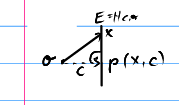
\includegraphics[width=5cm,height=5cm]{Beispiel 2.8}
 \end{figure}\\
\underline{Bsp.:} H()


\end{document}
